\chapter{Despliegue por defecto.} \label{cap:02Despliegue}

El despliegue de ATLAS en Docker es muy sencillo y está muy bien documentado en el repositorio de github de Broadsea \cite{githubBroadsea}.  Igualmente, en este manual se detallan nuevamente los pasos para la configuración y despliegue de la herramienta, añadiendo algunos pasos relevantes adicionales.

\section{Requisitos para el despliegue}

\begin{enumerate}
    \item Descargar e instalar Docker. Lo más sencillo es seguir las instrucciones de la \href{https://docs.docker.com/engine/install/}{página web oficial} para la descarga y seguir la configuración por defecto para la instalación.
    
    \item Descargar e instalar Git. Lo más sencillo es seguir las instrucciones de la \href{https://git-scm.com/downloads}{página web oficial} para la descarga y seguir la configuración por defecto para la instalación.
\end{enumerate}

\section{Deployment} \label{cap:02Deployment}

En este primer despliegue rápido de ATLAS, se desplegarán las configuraciones por defecto de la herramienta, siguiendo la guía de implementación rápida \textit{(Quick Start)} del repositorio de github.

\begin{enumerate}
    \item Por tanto, el primer paso para desplegar ATLAS es clonar localmente el repositorio de github de Broadsea. Una forma rápida de hacerlo es copiar la siguiente línea de código en el \code{cdm}.

\begin{lstlisting}[language=sh]
        git clone https://github.com/OHDSI/Broadsea.git
\end{lstlisting}

    \item El segundo paso, es desplegar el contenedor docker. Para ello, situar el puntero del \code{cdm}, en la carpeta donde se ha copiado el repositorio de github de Broadsea.

\begin{lstlisting}[language=sh]
        cd ruta\del\repositorio\Broadsea\local
\end{lstlisting}

    Una vez situado en la carpeta raíz del repositorio, se jecuta el comando que instalará y desplegará el perfil por defecto del contenedor docker en la máquina local.

\begin{lstlisting}[language=sh]
    docker compose pull && docker-compose --profile default up -d
\end{lstlisting}

\end{enumerate}

%--------------

\section{Comprobación de despliegue correcto} 

Se puede comprobar que se ha instalado correctamente el contenedor de Broadsea en la máquina local de distintas formas, tal y como se presenta a continuación.

\begin{enumerate} 

    \item La forma más sencilla de interactuar con el contenedor de Broadsea es a través de Docker Desktop. Ejecutando dicho programa, en la sección \textit{''containers"} se muestran todos los contenedores que están corriendo en el equipo. En este caso, debe aparecer un multi-contenedor llamado "broadsea" que contenga seis contenedores, tal y como se muestra en la Figura \ref{fig:dockerDesktop}.
    
\begin{figure}[H]
    \centering
    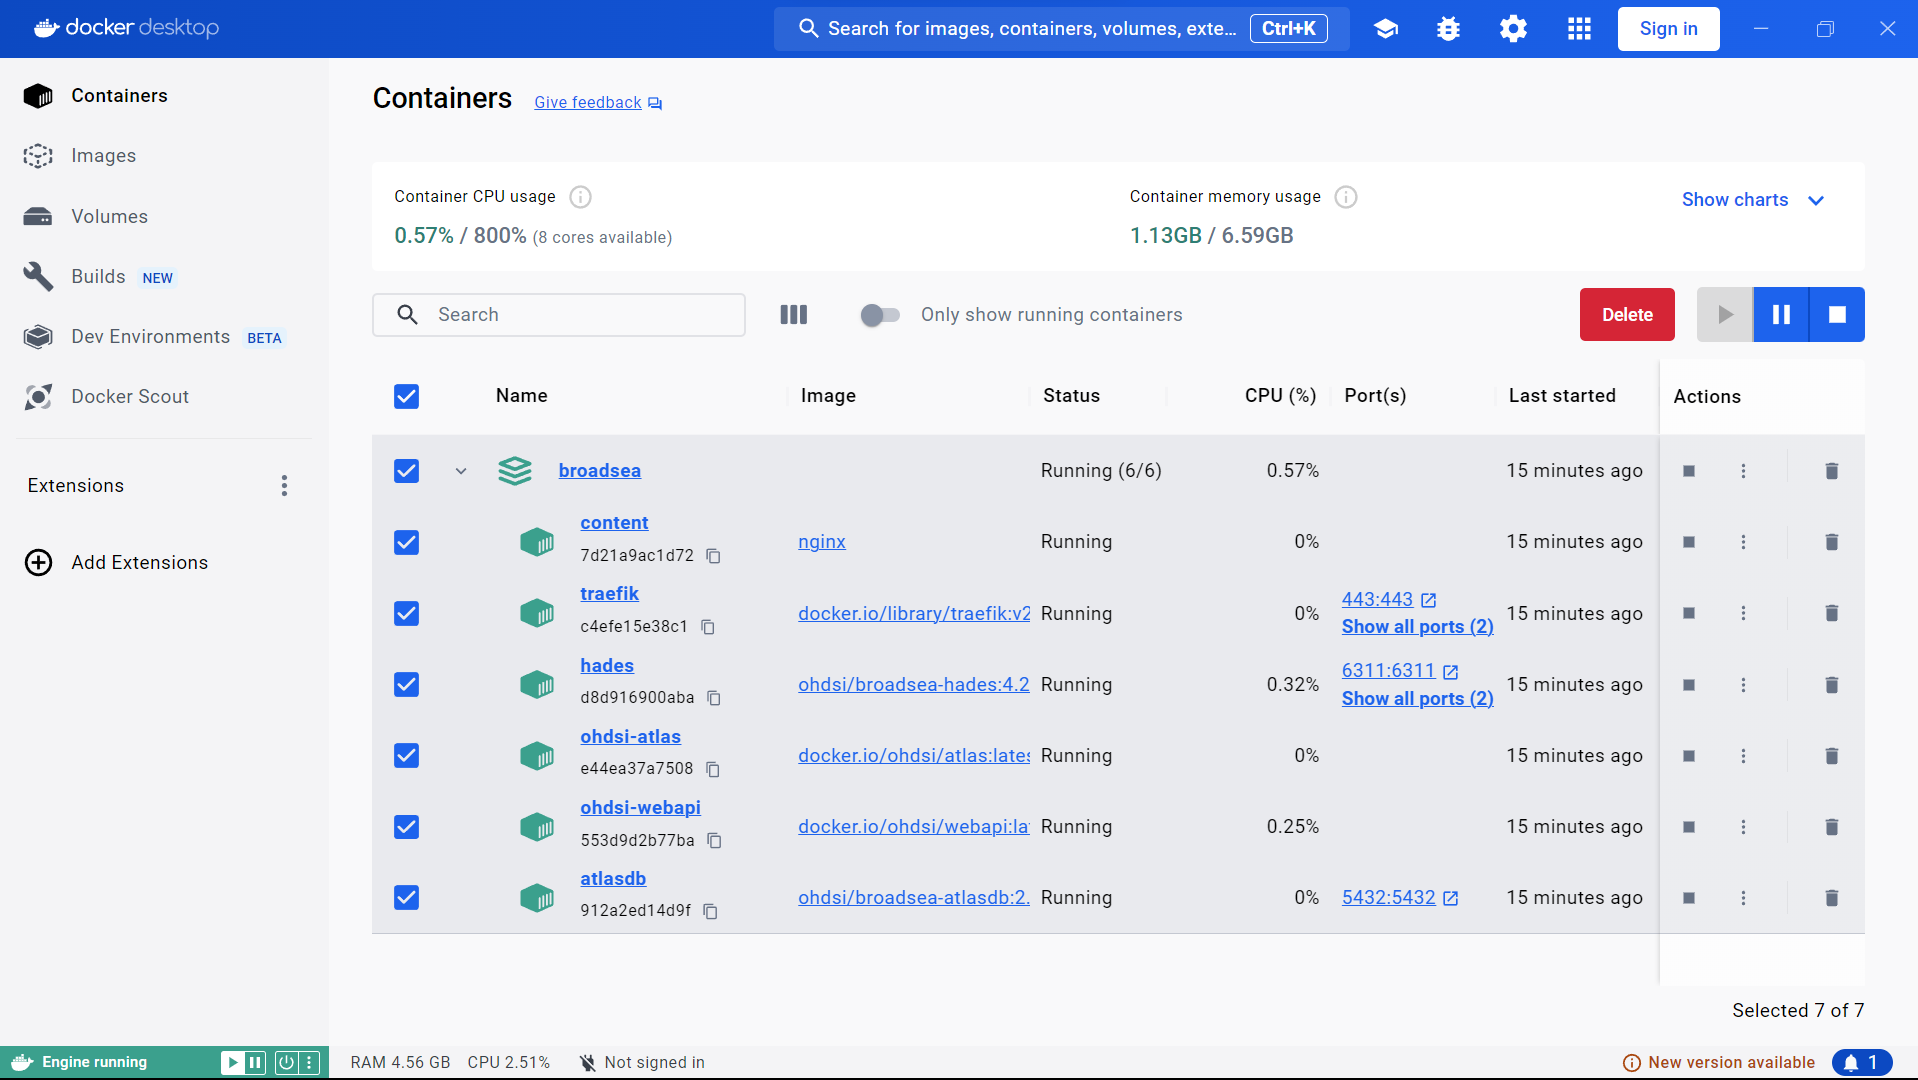
\includegraphics[width=0.90\textwidth]{figures/dockerDesktop.png}
    \caption{Captura de pantalla del contenedor Broadsea en Docker Desktop}
    \label{fig:dockerDesktop}
\end{figure}

    Mediante el panel de control de Docker se puede iniciar, pausar o detener cada contenedor (o todos a la vez) fácilmente y en cualquier momento. Por esto se dice que Broadsea ofrece servicios \textit{a-la-carte}.

    \item Otra forma de interactuar con el contenedor Docker es a través del \code{cmd}, ejecutando el comando \code{docker ps}, que muestra un listado de todos los contenedores que está ejecutando la máquina local. Con esta estrategia deberían mostrarse igualmente los mismos seis contenedores pertenecientes a broadsea, tal y como se muestra en la Figura \ref{fig:dockerCMD}

\begin{figure}[H]
    \centering
    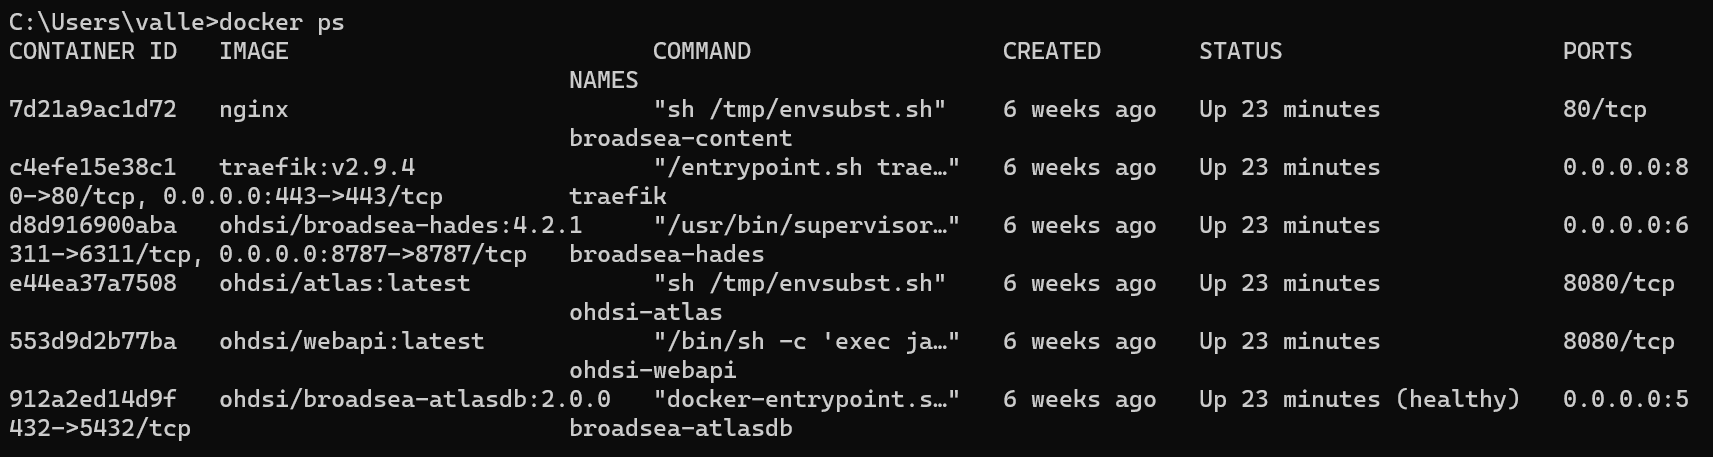
\includegraphics[width=0.90\textwidth]{figures/dockerCMD.png}
    \caption{Captura de pantalla del comando \code{docker ps } en el \code{cmd}}
    \label{fig:dockerCMD}
\end{figure}
    
    \item Por último, para acceder a los servicios de Broadsea hay que abrir en el navegador web (Chrome recomendado) el servidor en el que se alojan los servicios. Por defecto, Broadsea se aloja en el servidor 127.0.0.1, introducirlo en el navegador para explorar las herramientas del contenedor, tal y como se muestra en la Figura \ref{fig:broadseaCap}.

    \begin{figure}[H]
    \centering
    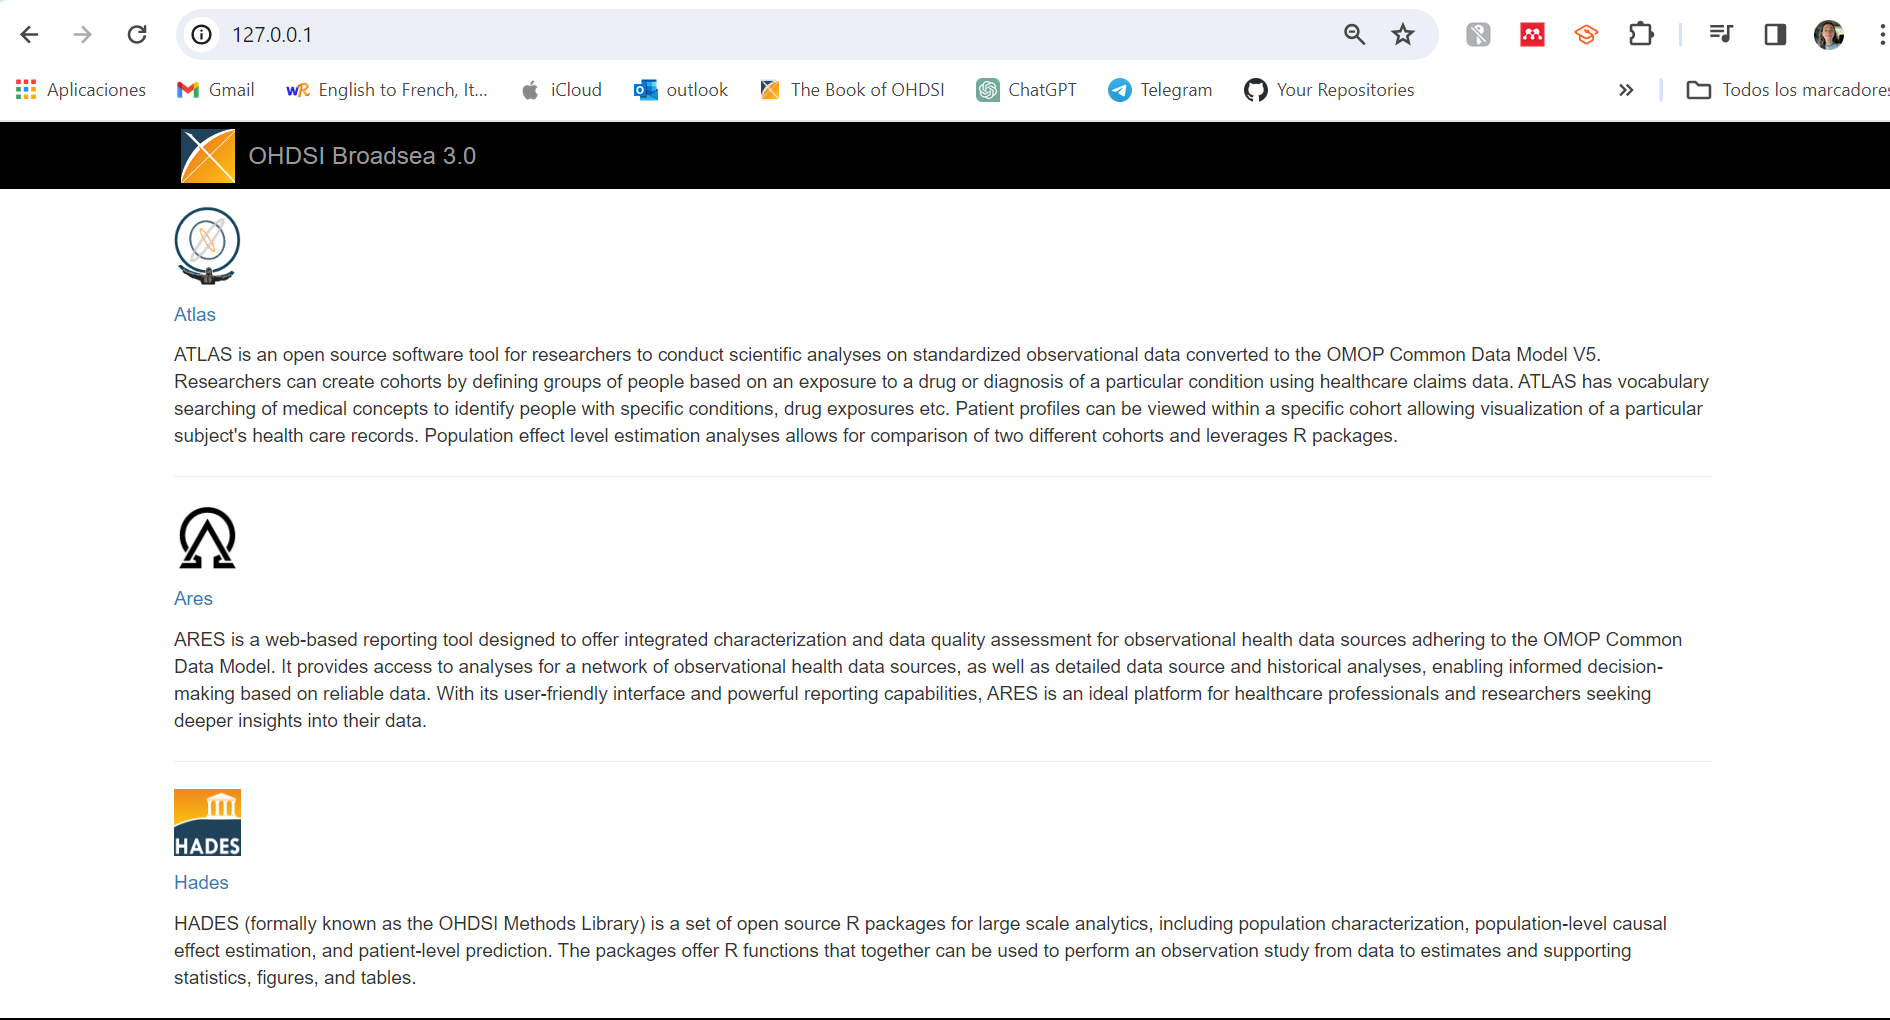
\includegraphics[width=0.90\textwidth]{figures/broadseaCap.png}
     \caption{Captura de pantalla del servidor Broadsea ejecutado en Chrome}
    \label{fig:broadseaCap}
\end{figure}
    
    Se puede comprobar o modificar el servidor exacto dónde se aloja el contenedor revisando el parámetro \code{BROADSEA\_HOST} de la sección 1 del archivo \code{.env} de la ruta local del repositorio. 

\begin{lstlisting}[language=sh]
###################################################
# Section 1:
# Broadsea Host
###################################################
DOCKER_ARCH="linux/amd64" # change this to linux/arm64 if using Mac Silicon, otherwise keep as-is
BROADSEA_HOST="127.0.0.1" # change to your host URL (without the http part)
HTTP_TYPE="http" # if using https, you need to add the crt and key files to the ./certs folder
BROADSEA_CERTS_FOLDER="./certs" 
\end{lstlisting}

    En este caso, no se modifica el servidor durante la configuración de Broadsea, por lo que de aquí en adelante la dirección del contenedor se aloja en el servidor \code{127.0.0.1}, tal y como se muestra en la Figura \ref{fig:broadseaCap}
   



    Es interesante notar que Broadsea permite el acceso interactivo a la herramienta Atlas, que es la que nos interesa en este caso, pero también a Ares y a Hades, otras dos herramientas muy relacionadas.

    La ejecución de ATLAS en Broadsea es similar a ATLAS demo, aunque con algunas diferencias. En primer lugar, Broadsea solo ejecuta, por defecto, una base de datos, que es la base de datos de Eunomia.

\begin{figure}[H]
    \centering
    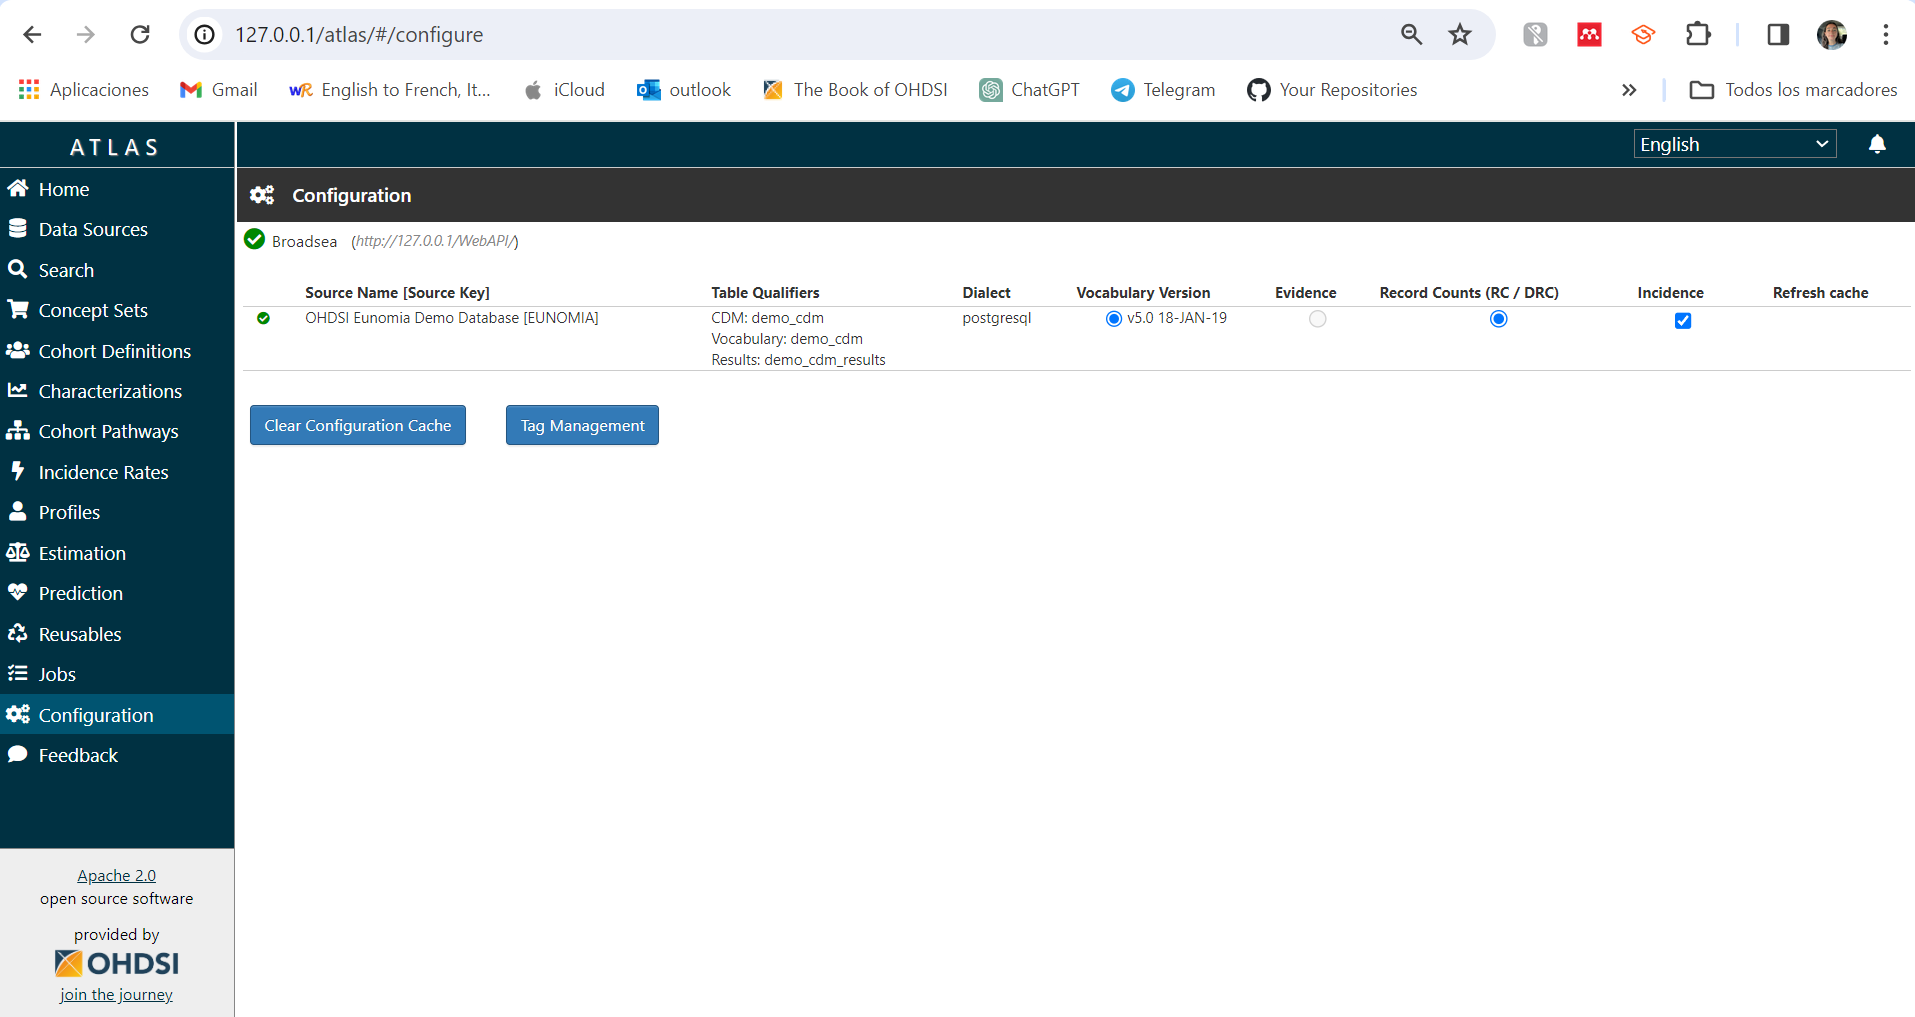
\includegraphics[width=0.90\textwidth]{figures/atlasBroadseaDB.png}
     \caption{Captura de pantalla de base de datos que utiliza ATLAS Broadsea}
    \label{fig:atlasBroadseaDB}
\end{figure}

    Por otra parte, y en contraste con la versión demo, ya no aparecen las entradas y estructuras que generan otros usuarios. La herramienta se presenta vacía, para ser completada solo con la información que nosotros introduzcamos.

\begin{figure}[H]
    \centering
    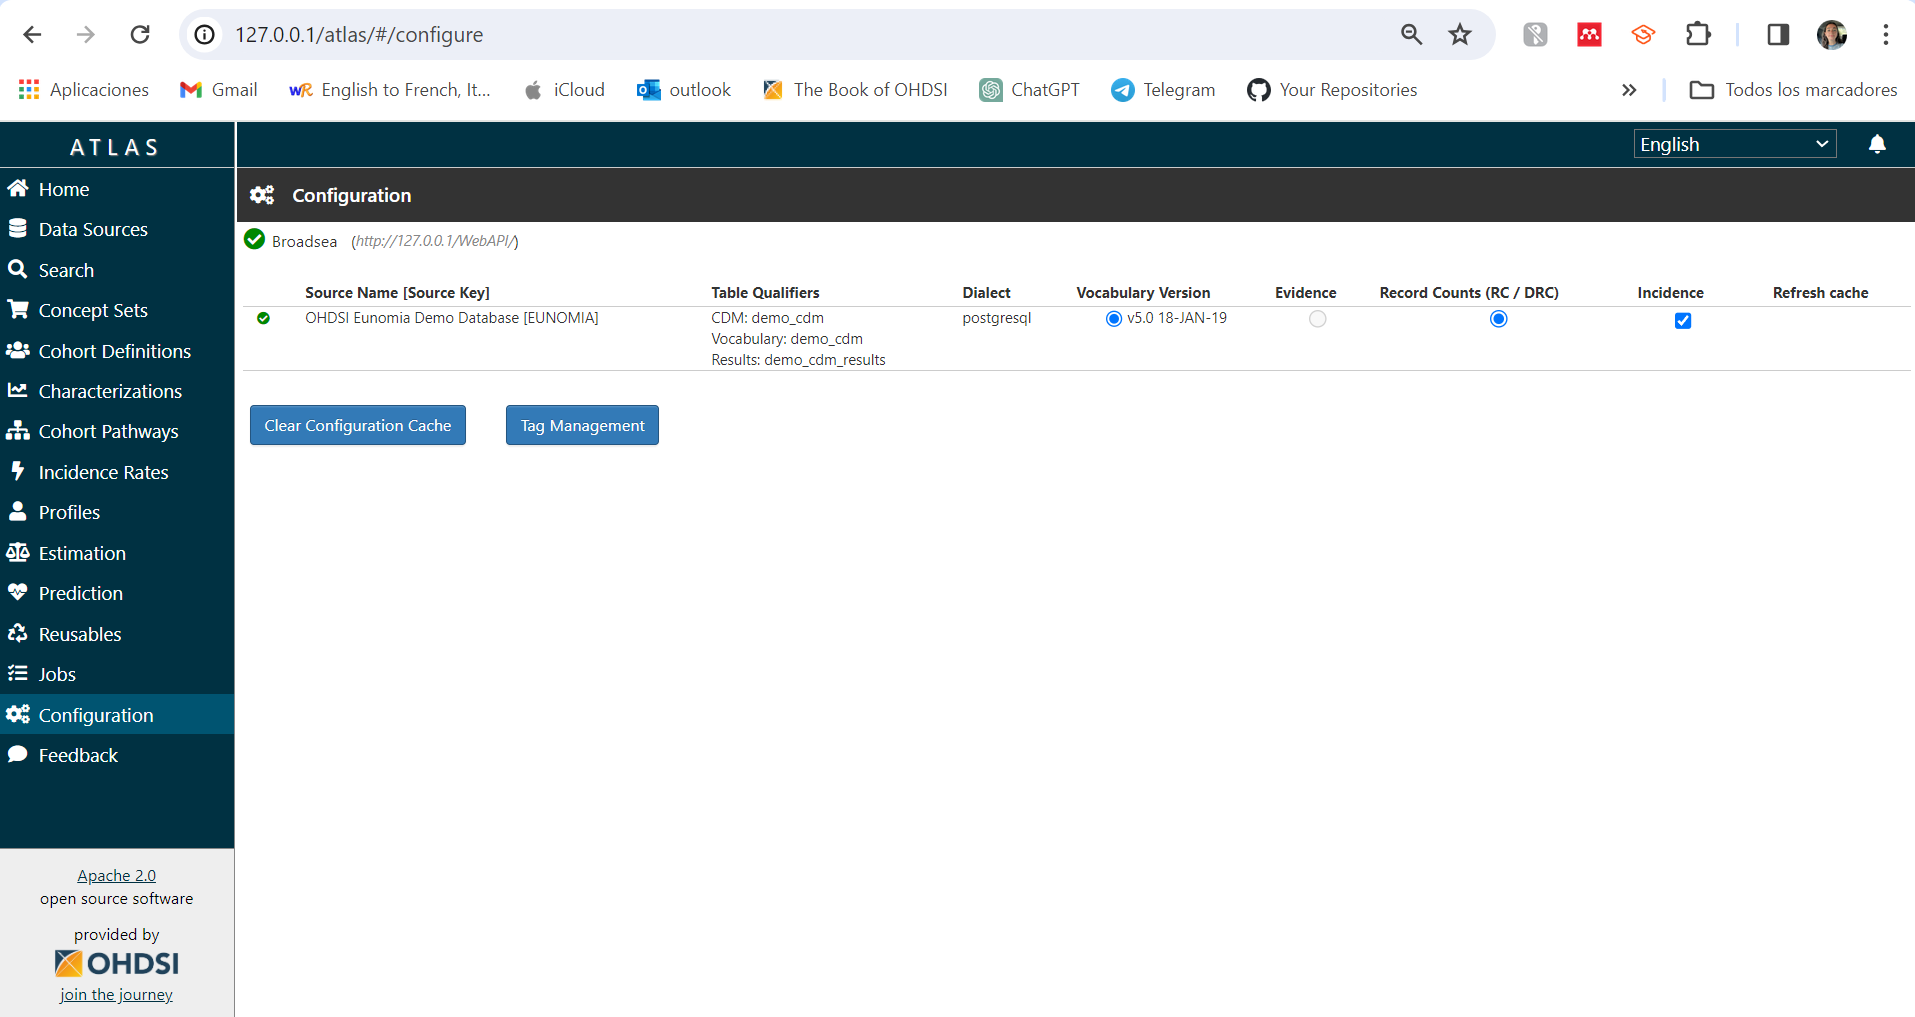
\includegraphics[width=0.90\textwidth]{figures/atlasBroadseaDB.png}
     \caption{Captura de pantalla señalando el número de entradas de definición de cohorte que almacena ATLAS Broadsea}
    \label{fig:atlasBroadseaDB}
\end{figure}
    
\end{enumerate}

\section{Solución de posibles errores}

\subsubsection{Error: Application initialization failed. Unable to connect to an instance of the WebAPI. Please contact your administrator to resolve this issue.}

El error aparece al dirigirse al servidor de Broadsea en el navegador.

\begin{figure}[H]
    \centering
    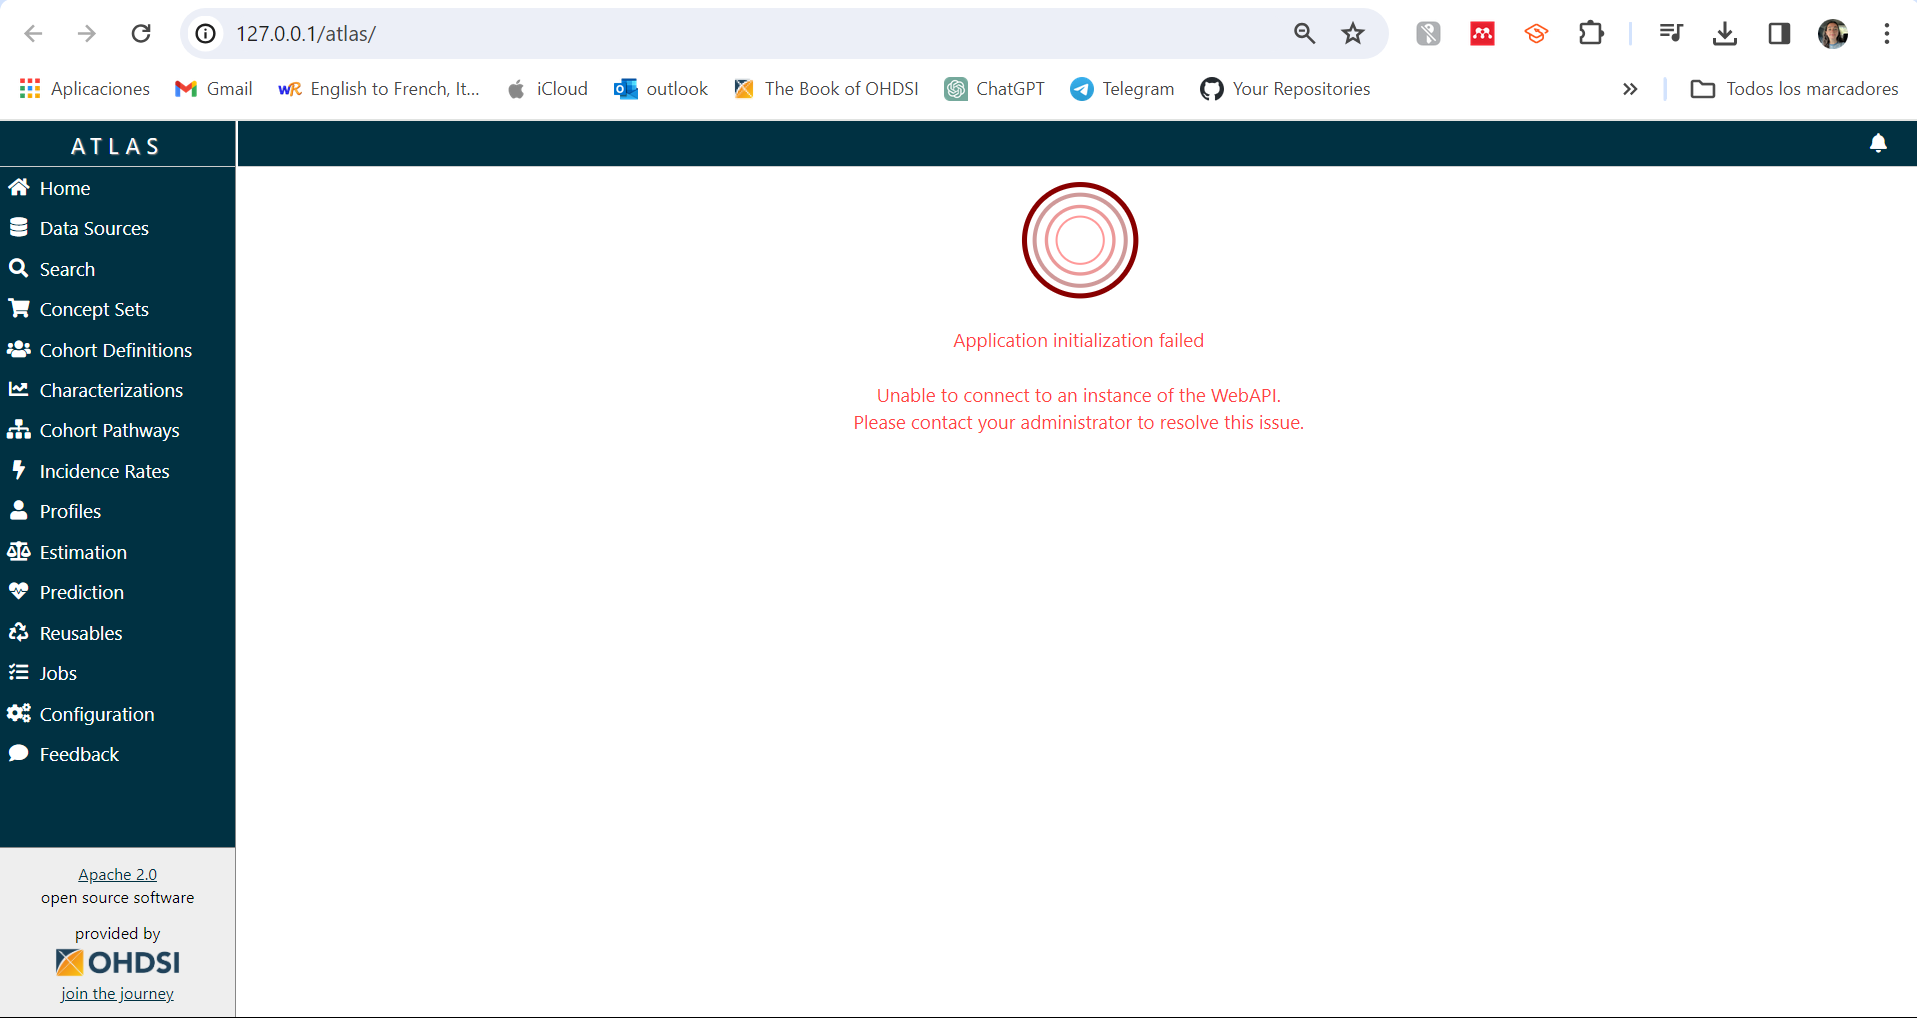
\includegraphics[width=0.90\textwidth]{figures/Error02AppFailed.png}
     \caption{Captura de pantalla del error}
    \label{fig:Error02AppFailed}
\end{figure}

Solución: Comprobar que todos los contenedores de docker implicados están corriendo. Recargar varias veces la página.


